% Source ownership:
% - Itxaso 

% ============================================================
\section{Initial Configuration Generation}
\label{sec:initial_conf}
% ============================================================

\subsection{Internal-Coordinate Builder}

The \texttt{initial\_conf} module is responsible for generating the starting
conformation of the polyethylene chain. The builder uses a recursive
internal-coordinate approach: each successive carbon atom is placed by
specifying a fixed C--C bond length ($d = 1.54\,\text{\AA}$), a fixed C--C--C
bond angle ($\theta = 114^\circ$), and a selectable dihedral angle $\phi$.
A hard-sphere overlap check with threshold $r_{\min} = 2.0\,\text{\AA}$ is
performed after each placement to avoid unphysical self-intersections during
chain construction.

\begin{lstlisting}[caption={Core internal-coordinate placement loop in \texttt{initial\_conf.f90}.}]
! Place carbon i based on the last two accepted positions
do i = 4, n_carbons
  ! Bond vector from i-2 to i-1 (normalised)
  b1 = coords(i-1,:) - coords(i-2,:)
  b1 = b1 / vnorm(b1)

  ! Normal to the C(i-2)-C(i-1)-C(i) plane
  b0 = coords(i-2,:) - coords(i-3,:)
  n_vec = cross(b0, b1)
  if (vnorm(n_vec) > 1.0d-8) n_vec = n_vec / vnorm(n_vec)

  ! Proposed new position using dihedral phi
  d_vec = bond_length * (                          &
      -cos_theta * b1                              &
      + sin_theta * (cos_phi * n_vec               &
                   + sin_phi * cross(b1, n_vec)))

  candidate = coords(i-1,:) + d_vec

  ! Overlap check against all previously placed atoms
  overlap = .false.
  do j = 1, i-1
    if (vnorm(candidate - coords(j,:)) < r_min) then
      overlap = .true.
      exit
    end if
  end do
  if (.not. overlap) coords(i,:) = candidate
end do
\end{lstlisting}

When explicit hydrogens are requested (\texttt{explicit\_h = .true.}), two
hydrogen atoms are appended for each internal CH$_2$ group and one for each
terminal CH$_3$ group, giving $N_{\text{atoms}} = 3N_C + 2$ total atoms for
a chain of $N_C$ carbons. The hydrogen placement is based on a local tetrahedral
frame: instead of placing the H atoms coplanar with the C--C--C backbone (chemically inconsistent), they are positioned out of the
backbone plane at the correct tetrahedral angle of $\approx 109.5^\circ$.

\begin{lstlisting}[caption={Out-of-plane hydrogen placement for internal CH$_2$ groups.}]
! For each internal carbon i (not first or last):
! Build local orthonormal frame {b_fwd, perp, out_of_plane}
b_fwd = coords(i+1,:) - coords(i-1,:)
b_fwd = b_fwd / vnorm(b_fwd)

! Perpendicular to backbone, in the C(i-1)-C(i)-C(i+1) plane
b_back = coords(i-1,:) - coords(i,:)
b_back = b_back / vnorm(b_back)
perp   = b_back - sum(b_back*b_fwd)*b_fwd
if (vnorm(perp) > 1.0d-8) perp = perp / vnorm(perp)

! Out-of-plane direction (cross product)
out_of_plane = cross(b_fwd, perp)
out_of_plane = out_of_plane / vnorm(out_of_plane)

! Place H1 and H2 symmetrically out of plane (tetrahedral geometry)
! cos(109.5 deg) ~ -1/3  =>  sin(109.5 deg) ~ sqrt(8/9)
h1 = coords(i,:) + r_CH * ( (-1.0d0/3.0d0)*(-perp)  &
     + sqrt(8.0d0/9.0d0) * 0.5d0 * ( out_of_plane + b_fwd) )
h2 = coords(i,:) + r_CH * ( (-1.0d0/3.0d0)*(-perp)  &
     + sqrt(8.0d0/9.0d0) * 0.5d0 * (-out_of_plane + b_fwd) )
\end{lstlisting}

\subsection{Configuration Modes}

Five distinct initial configuration modes have been implemented, each designed
to probe a different region of the polymer's conformational space:

\begin{table}[h!]
\centering
\caption{Summary of implemented initial configuration types.}
\label{tab:conf_types}
\begin{tabular}{clp{9cm}}
\toprule
\texttt{conf\_type} & Name & Description \\
\midrule
1 & All-trans (planar) & All dihedrals set to $\phi = 0^\circ$; fully extended
                         zigzag chain. Maximum end-to-end distance. \\
2 & Random & Each dihedral drawn uniformly from $[-\pi,\,\pi]$; maximally
             disordered starting state. \\
3 & RIS-like discrete & Dihedrals assigned with probabilities reflecting the
                        Rotational Isomeric State model (trans, gauche$^+$,
                        gauche$^-$). \\
4 & Spring / helix & Progressive dihedral increment per bond, producing a
                     helical backbone (proposed by ai-murphy). \\
5 & Perturbed trans & Small random perturbation applied to the all-trans
                      geometry; slight out-of-plane deviation while remaining
                      close to the global minimum. \\
\bottomrule
\end{tabular}
\end{table}

\begin{figure}[h!]
  \centering
  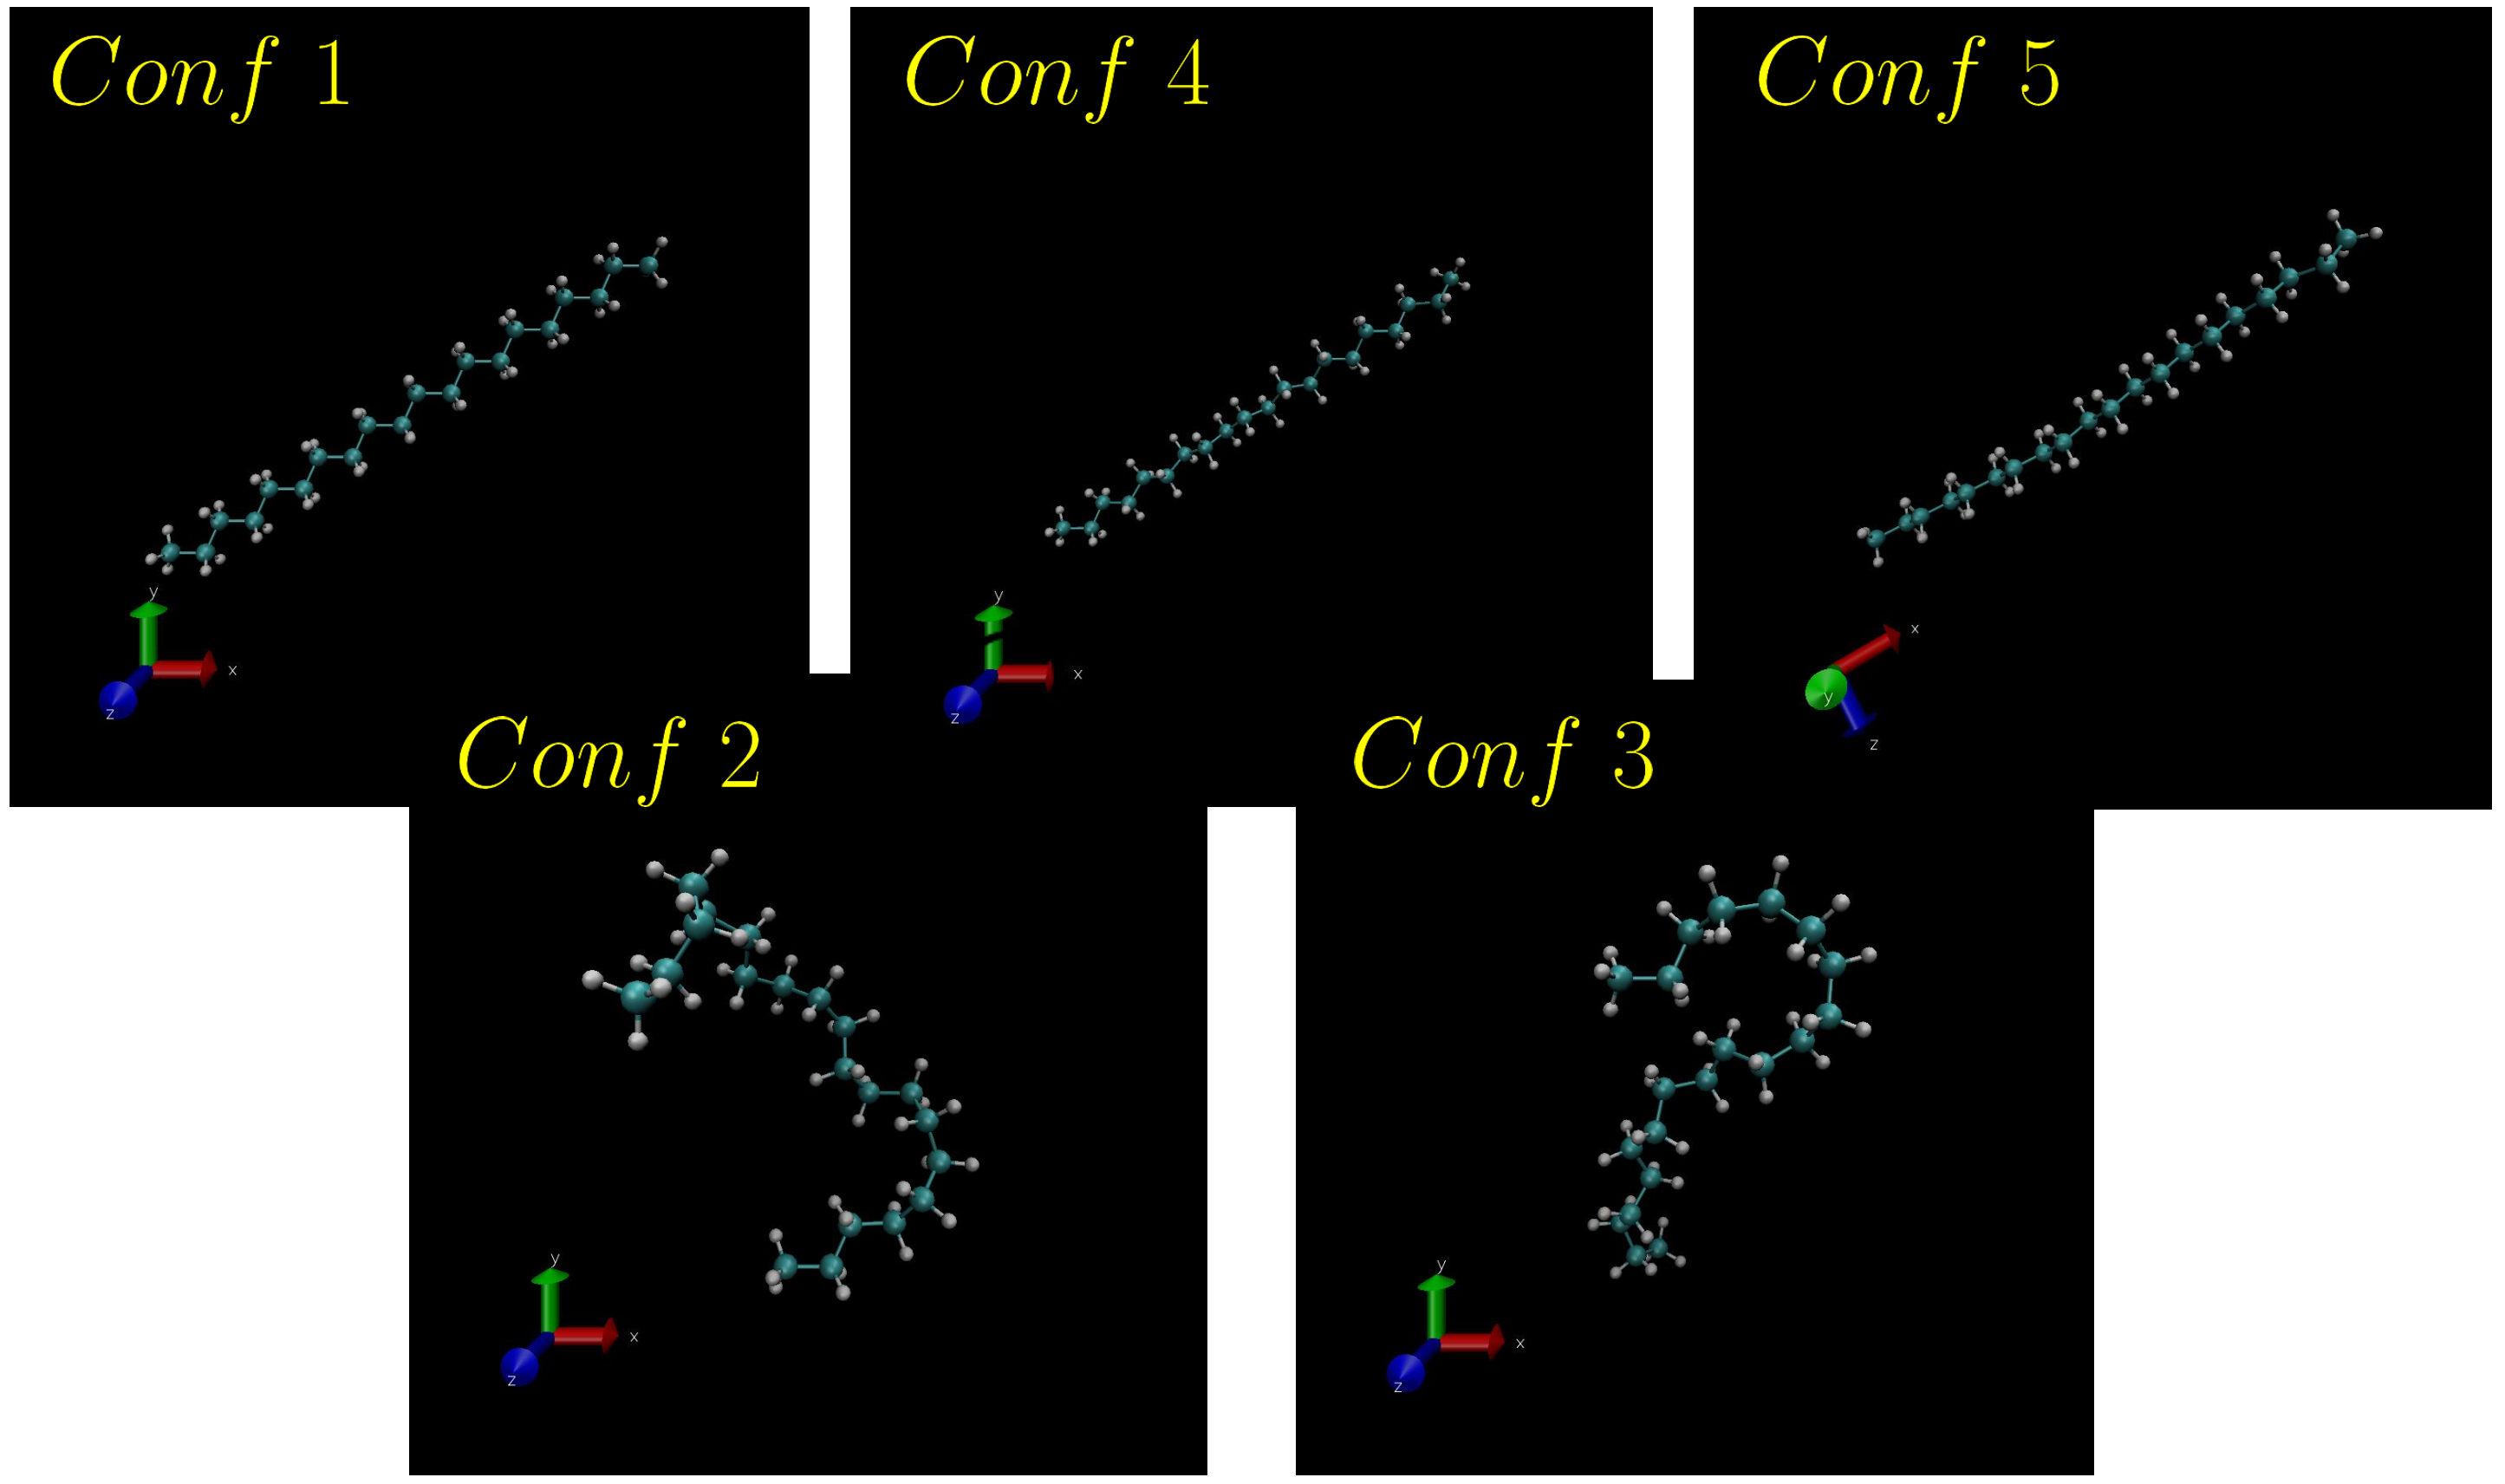
\includegraphics[width=\textwidth]{figs/INITIAL-CONFIGS.png}
  \caption{VMD snapshots of the five implemented initial configuration modes
  for the polyethylene chain. From left to right: (1) all-trans planar,
  (2) random, (3) RIS-like discrete, (4) spring/helix, and
  (5) perturbed trans.}
  \label{fig:initial_configs}
\end{figure}

Configurations 1 and 5 span the near-trans region of phase space, whereas
configurations 2 and 3 provide disordered starting points. Configuration 4 was
added to test helical initial geometries. Figure~\ref{fig:initial_configs}
provides a direct visual comparison of these starting states, illustrating the
broad structural diversity used to initialize the simulations.

This variety is relevant when the simulation is tested at different
temperatures: some initial states may lie closer to the equilibrated ensemble
than others, reducing the effective burn-in time.

% ============================================================